\begin{frame}
    \frametitle{Transportwegverschlüsselung}
    \begin{center}
      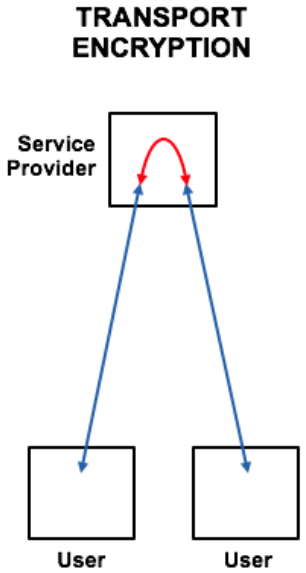
\includegraphics[height=0.8\textheight]{../../img/enc-transport.png}
    \end{center}
\end{frame}

\note{TLS, besser bekannt unter dem alten Namen SSL, ist eine TRANSPORTWEG-Verschlüsselung. D.h. dass die Daten auf dem Weg durchs Internet bis zum Server verschlüsselt sind, auf dem Server aber unverschlüsselt liegen. Dies wird z.B. für Websites oder in Emailprogrammen fürs abholen und senden von Emails verwendet. Wenn man beispielsweise ein Foto bei Facebook hochlädt, dann ist dies auf dem Weg zum Facebookserver verschlüsselt, aber liegt dann auf dem Facebookserver wieder unverschlüsselt.}

\begin{frame}
    \frametitle{SSL im Browser}
    \begin{center}
      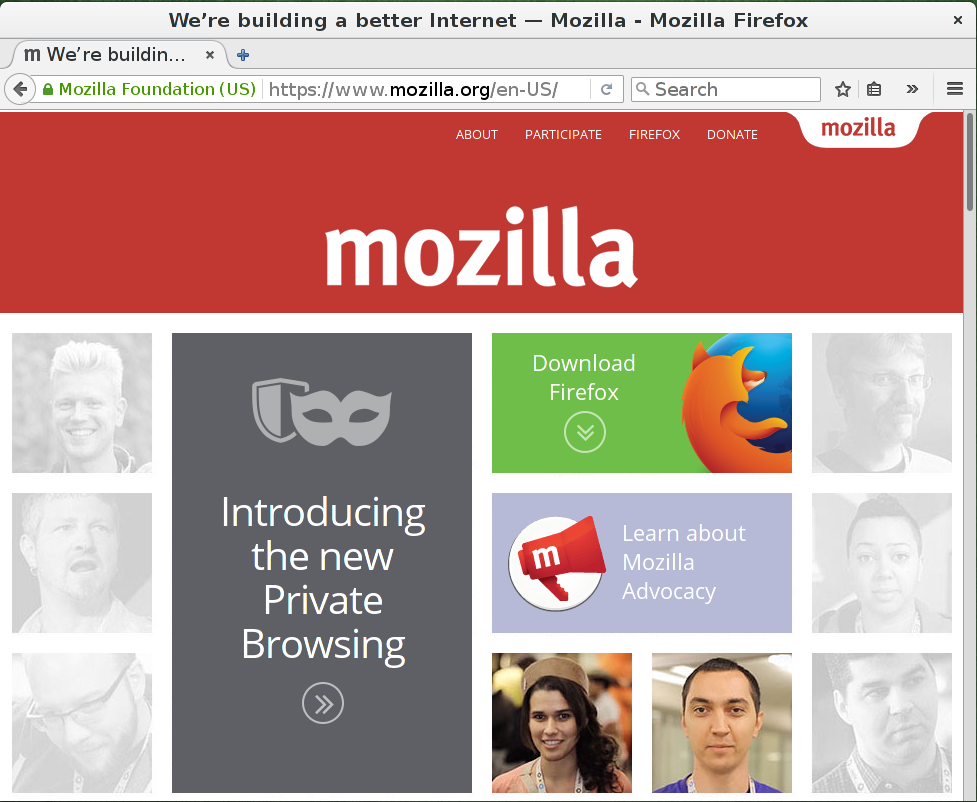
\includegraphics[height=0.7\textheight]{../../img/ssl_special.png}
    \end{center}
\end{frame}

\note{Im Firefox sieht das so aus, wenn man TLS benutzt. Überlicherweise zeigt der Browser dann ein Schloss vor oder hinter der URL an. Immer steht jedoch am Anfang der URL ein https statt einem einfachen http. Das s steht für secure und zeigt die Nutzung von TLS an. Dies sollte man insbesondere wenn man sich bei einer Website einloggt immer überprüfen, weil mit dem nichtverschlüsselten http auch das eigene Passwort dann unverschlüsselt übers Internet versendet wird - für jeden einfach einsehbar.}

\begin{frame}
    \frametitle{Ungültiges Zertifikat}
    \begin{center}
	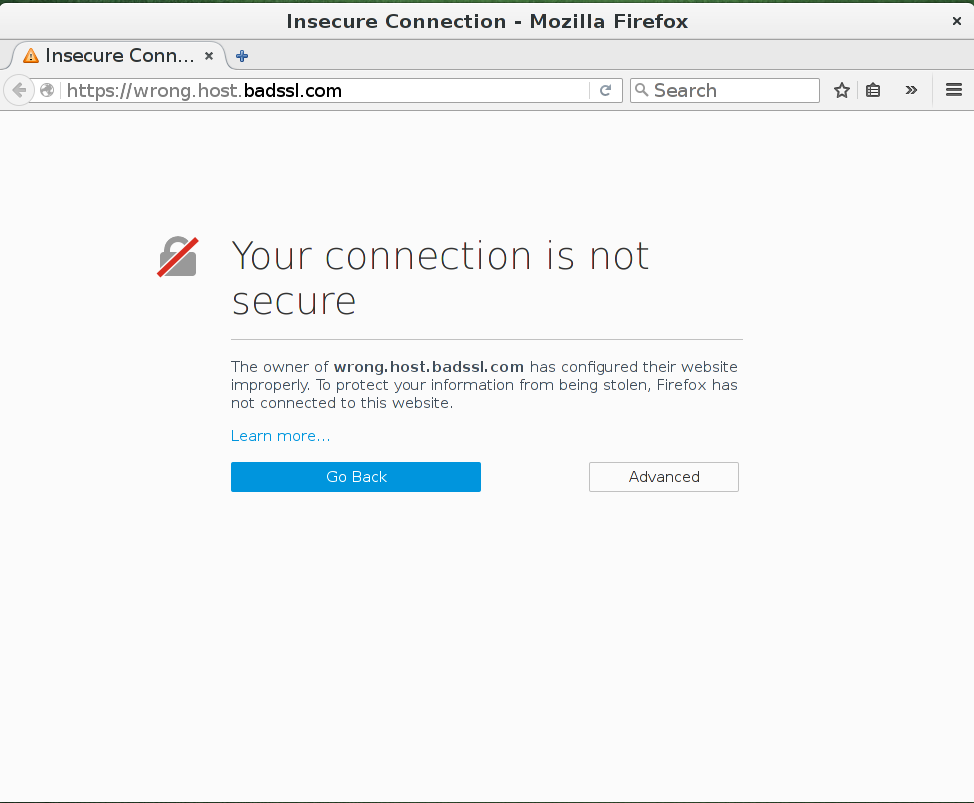
\includegraphics[height=0.7\textheight]{../../img/ssl_badcert.png}
    \end{center}
\end{frame}

\note{Wenn einem der Browser eine ``Zertifikatswarnung'' anzeigt, heißt das, dass die Verschlüsselung zwar besteht, es aber nicht sichergestellt ist, dass man wirklich mit der Website kommuniziert oder nicht etwa mit jemandem, der sich dazwischengeschummelt hat. So eine Warnung sollte man nicht ignorieren, sondern es besser später oder von einem anderen Rechner aus probieren.}
